\chapter{Evaluation}
\label{chap:evaluation}

We are now ready to evaluate the efficiency of our schedulers for heterogeneous systems, which are proposed in Chapter~\ref{chap:optimizedHeterogeneousScheduling} and~\ref{chap:schedulingHeuristics}. First, in Section~\ref{sec:inputs_generation} we describe the default experimental settings and the generation procedure for input programs parameters. Then, in Section~\ref{sec:scheduler_tool} we describe our C++ Scheduler tool, which we implemented to evaluate our schedulers. By using this tool, we conduct various experiments with numerous input programs and report the results in Section~\ref{sec:evaluation_scheduling}. In addition, to estimate the tractability scale for our tool, we also plot its computation time along with the experiments.


Experiments are run on a system with next specifications:
%
\begin{itemize}
\item Processor: AMD Ryzen 5 4600h @ 3.4GHz;
\item Cores: 6;
\item Caches:
\item[]
\begin{itemize}
\item L1: 64 KB (per core);
\item L2: 512 KB (per core);
\item L3: 8 MB (shared between cores);
\end{itemize}
\item Memory (RAM): 16 GB DDR4 @ 3200 MHz;
\item Operating system: Linux Mint 22 LTS;
\item Compiler: g++ 13.3;
\item Compiler flag: -O3 (all optimizations are enabled).
\end{itemize}




\section{Inputs generation}
\label{sec:inputs_generation}

\begin{table}
\captionsetup{justification=centering}
\caption{Key parameter values}
\centering
\begin{tabular}{l|p{28mm}} 
%\begin{tabular}{l|l|l} 
 \hline
 Parameter &  Values\\[1pt]
 \hline
Cores number, $m^{\mathsf{slow}} + m^{\mathsf{fast}}$ & $1+1$ \\[4pt]
Programs number, $N$ & 3 \\[4pt]
Total blocks number, $N^{\mathsf{blocks}}$ & 5 \\[6pt]
Block time, Core \{1,2\}, $t_{jm}$ & 1:\ [220; 250] 2:\ \ [210; 230]  \\[15pt]
Block energy use, Core \{1,2\}, $e_{jm}$ & 1:\ [120; 130] 2:\ \  [125; 150] \\
 \hline
\end{tabular}
\label{tab:defaultSettings}
\vspace{-5mm}
\end{table}


Input programs are generated for the key parameters listed in Table~\ref{tab:defaultSettings}, along with their default values and ranges. Their choice considers the assumption for the difference between cores speed and energy consumption. By ``Core 1" we denote a slow but energy-efficient core, and ``Core 2" \-- faster but energy-hungry. Then, the generation procedure for one input is the following:
%
\begin{enumerate}
\item Cores number is fixed to $m$;
\item Programs number $N$ is randomly picked;
\item Total blocks number for all programs in one input is fixed to $N^{\mathsf{blocks}}$, so that
\item $N^{\mathsf{blocks}}$ is randomly distributed between $N$ programs;
\item For every program $P_i$, its block $b_j$, core $m$, this block's requirements $t_{jm}$ and $e_{jm}$ for runtime and energy are randomly picked.
\end{enumerate}
%
All parameter values specified by ranges are picked according to a uniform distribution.

We note that programs requirements, like the ones listed in Table~\ref{tab:defaultSettings}, in practice are typically collected by using a suitable profiler tool, such as \textsc{perf}\footnote{https://perfwiki.github.io}. In each experiment the value of one of the parameters is varied, while other parameters are fixed to defaults. For each value of a varying parameter we generate at least 100 inputs and plot the average output value as a datapoint. All experiments assume a synchronous invocation of all programs at $t=0$.


\section{Scheduler implementation}
\label{sec:scheduler_tool}

All our schedulers are implemented by a C++ Scheduler tool. As an input, it takes values of programs parameters, as discussed above. Then it traverses the state-transition graph in a depth-first way, and at the end produces optimal and suboptimal schedules. The tool outputs various summarized statistics regarding computed schedules. Currently the tool does not support migration and preemption overheads, which are to be included.

In Fig.~\ref{fig:screenshots} we depict the screenshots of using our tool through the Terminal:
%
\begin{enumerate}
\item Specification of input parameters: Fig.~\ref{fig:inputScreen};
\item Verbosed graph states traversal: Fig.~\ref{fig:blockLogScreen};
\item Results output: Fig.~\ref{fig:outputScreen}.
\end{enumerate}

Our Scheduler tool is available on demand.

\begin{figure*}
    \centering
    \begin{subfigure}{0.32\textwidth}
        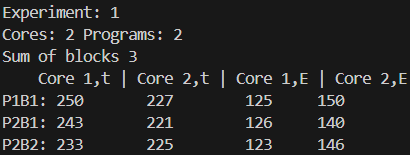
\includegraphics[width=\linewidth]{figs/inputScreen.png}
        \caption{Input specification}
        \label{fig:inputScreen}
    \end{subfigure}
    \hspace{3mm}
     \begin{subfigure}{0.24\textwidth}
        \includegraphics[width=\linewidth]{figs/OutputScreen.png}
        \caption{Output statistics}
        \label{fig:outputScreen}
    \end{subfigure} 
        \hspace{3mm}
     \begin{subfigure}{0.33\textwidth}
        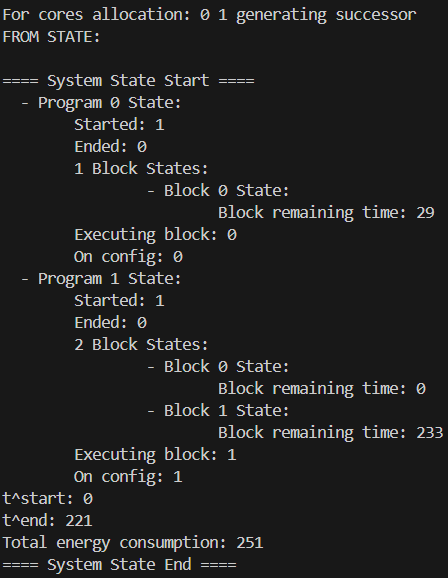
\includegraphics[width=\linewidth]{figs/blockLogScreen.png}
        \caption{Intermediate graph state}
        \label{fig:blockLogScreen}
    \end{subfigure}
     \caption{Scheduler tool use: screenshots}
     \label{fig:screenshots}
\end{figure*}

\section{Schedulers evaluation}
\label{sec:evaluation_scheduling}

Finally we compare the performance of our schedulers:
%
\begin{itemize}
\item optimal, which is determined by brute-forcing (Chapter~\ref{chap:optimizedHeterogeneousScheduling});
\item a random-walk with a customizable number of runs (Section~\ref{sec:randomWalk}),
\item a greedy walk (Section~\ref{sec:greedyWalk}).
\end{itemize}
%

The key performance metric for schedulers comparison is EDP $\uprho$ (see Section~\ref{sec:energyDelayProduct}) and programs response times $t^\mathsf{RT}$ (see Section~\ref{sec:timePerformanceMetrics}). We also assess the Scheduler tool runtime $t$.



\subsection*{Experiment: Varying blocks number}

The first experiment is for a varying total number of programs blocks $N^\mathsf{blocks}$. In fact, the $N^\mathsf{blocks}$ parameter makes the most significant impact on the performance difference between schedulers.

In Fig.~\ref{fig:EDPVsBlocks} and~\ref{fig:BlockEDPVsBlocks} we report the dependency between EDP $\uprho$ and $N^\mathsf{blocks}$. We observe that the 100-random walk heuristic is near-optimal, but computed significantly faster, as seen in Fig.~\ref{fig:RuntimeVsBlocks}. Regarding other schedules, the single random walk and the greedy heuristics result in significantly higher EDP, meaning that the schedules they produce consume higher energy. The deviation between the EDP most and least efficient schedules is up to 40-50\% for $N^\mathsf{blocks} = 12$, and seems to increase further with $N^\mathsf{blocks}$.

In turn, computed average programs response times are in Fig.~\ref{fig:RTVsBlocks} and~\ref{fig:BlockRTVsBlocks}. We observe nearly the same trends as for EDP.

The computation time for an optimal schedule is exponential, unlike heuristics, according to Fig.~\ref{fig:RuntimeVsBlocks} (note the logarithmic scale for the time axis).

\begin{figure*}
    \centering
    \begin{subfigure}{0.4\textwidth}
        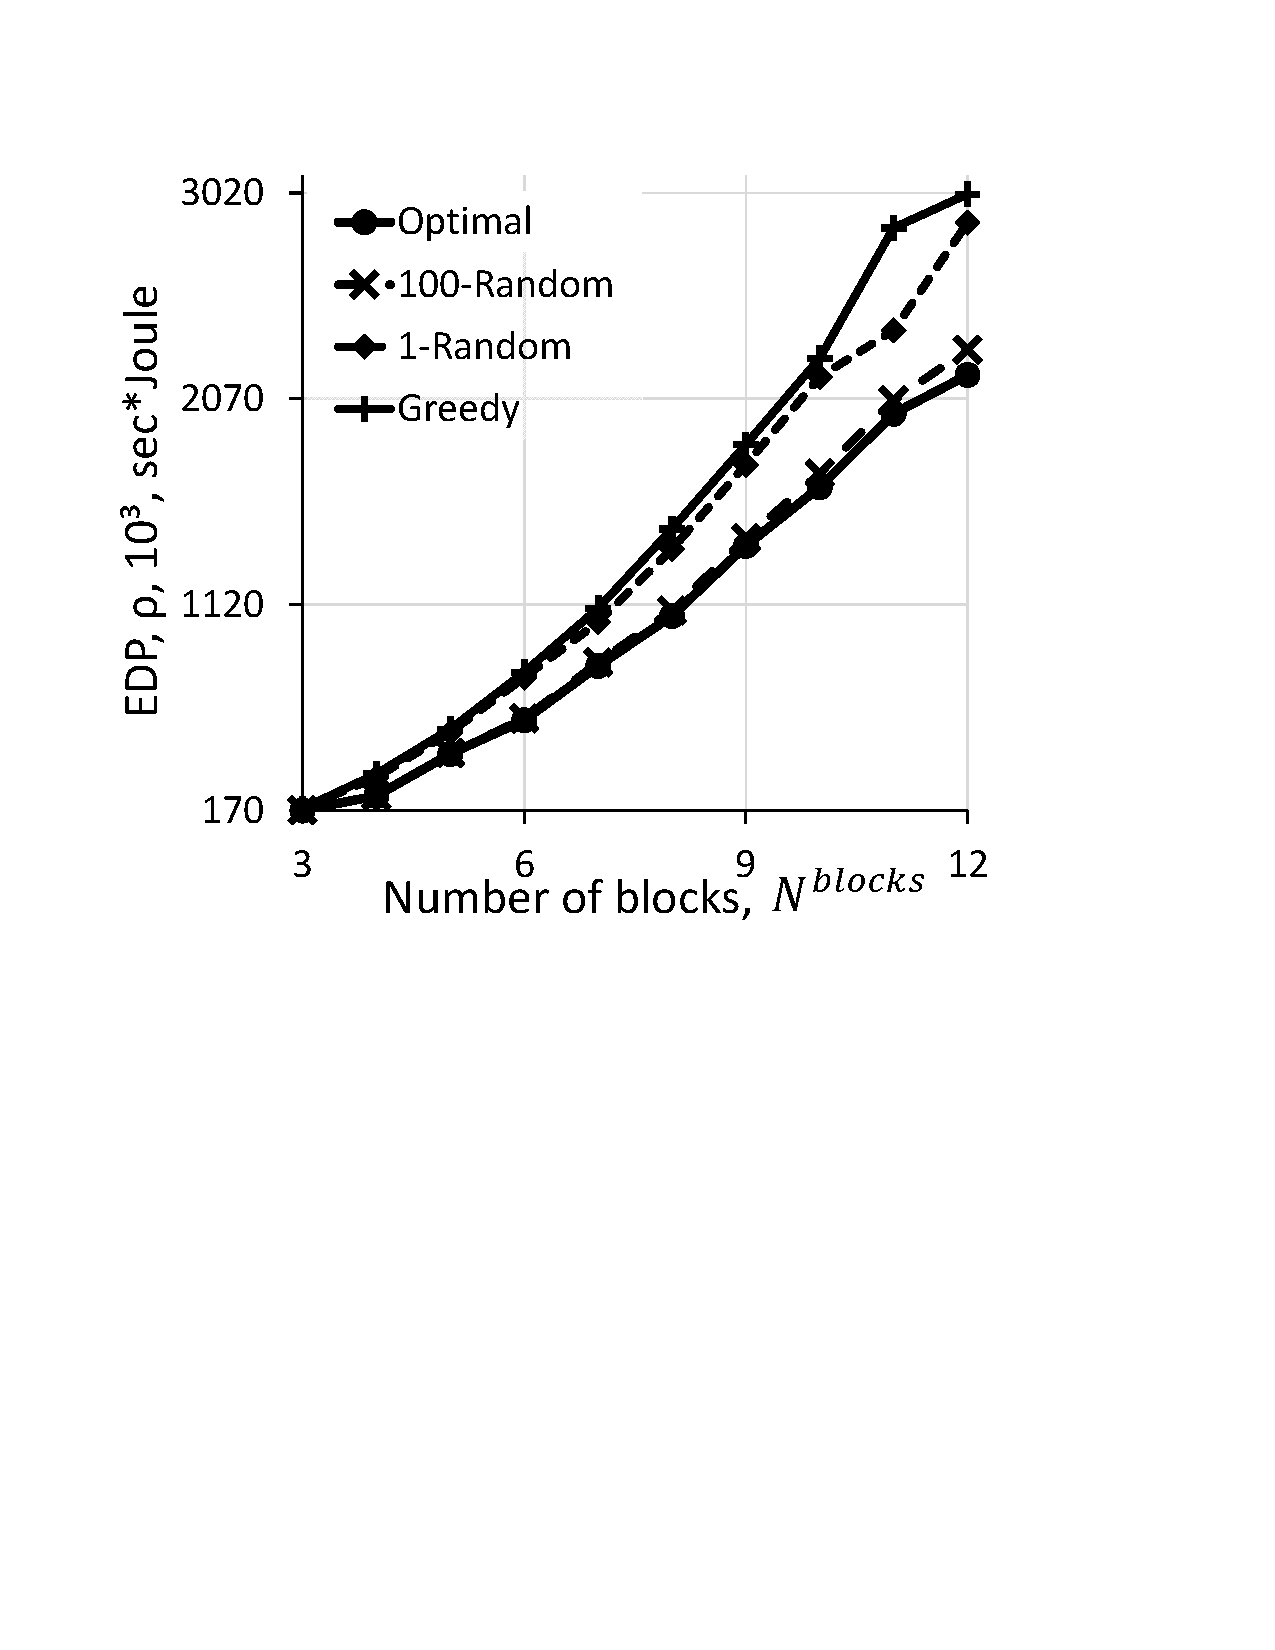
\includegraphics[width=\linewidth]{figs/EDPVsBlocks.pdf}
        \caption{EDP vs. blocks number}
        \label{fig:EDPVsBlocks}
    \end{subfigure}
    \hspace{13mm}
     \begin{subfigure}{0.4\textwidth}
        \includegraphics[width=\linewidth]{figs/RTVsBlocks.pdf}
        \caption{Response time vs. blocks number}
        \label{fig:RTVsBlocks}
    \end{subfigure}
     \caption{Varying blocks number: greedy, random walk and optimal schedules EDP and response times}
       \label{fig:varyingBlocks}
\end{figure*}

\begin{figure*}
    \centering
     \begin{subfigure}{0.4\textwidth}
        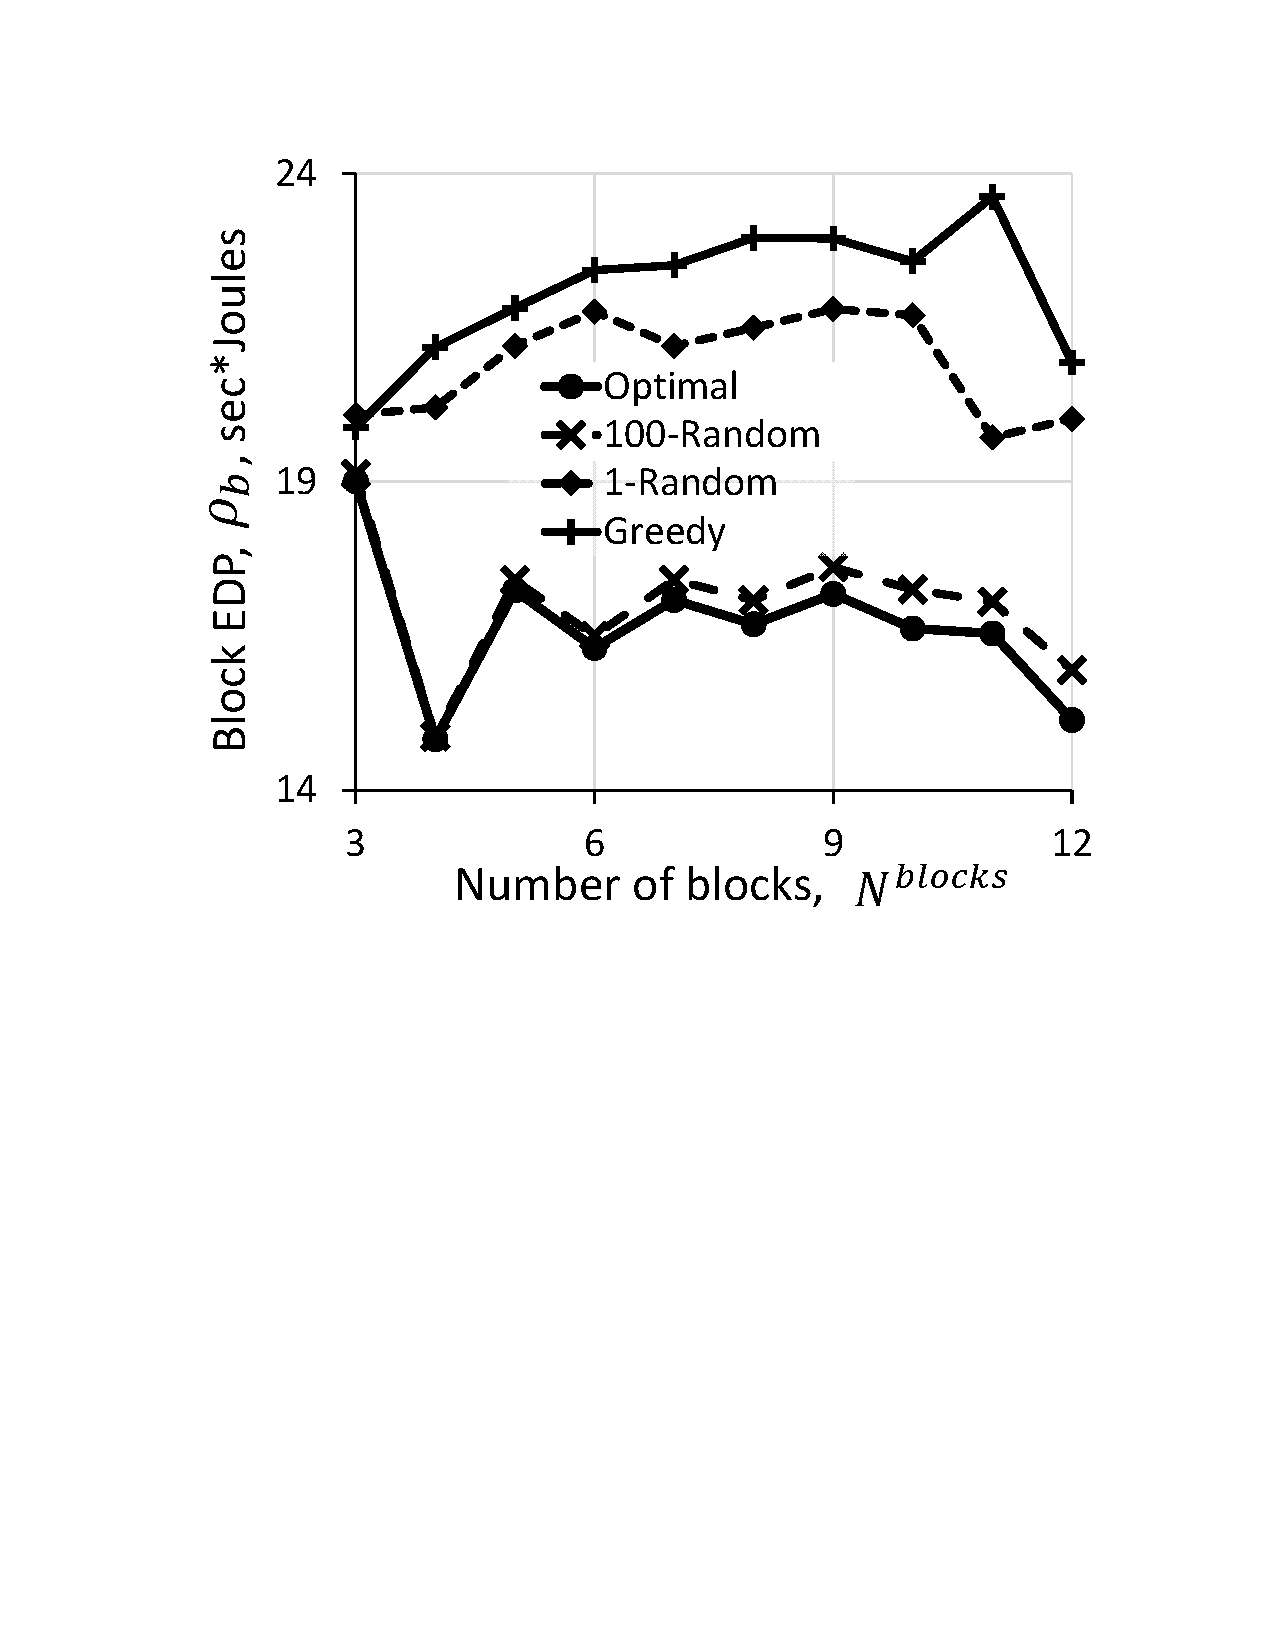
\includegraphics[width=\linewidth]{figs/BlockEDPVsBlocks.pdf}
        \caption{Per block EDP vs. blocks number}
        \label{fig:BlockEDPVsBlocks}
    \end{subfigure}
    \hspace{12mm}
     \begin{subfigure}{0.4\textwidth}
        \includegraphics[width=\linewidth]{figs/BlockRTVsBlocks.pdf}
        \caption{Per block response time vs. blocks number}
        \label{fig:BlockRTVsBlocks}
    \end{subfigure}
    \caption{EDP and runtime per block vs number of blocks. Continuation of Fig.~\ref{fig:varyingBlocks}.}
\end{figure*}



\begin{figure*}
    \centering
    \begin{subfigure}{0.38\textwidth}
        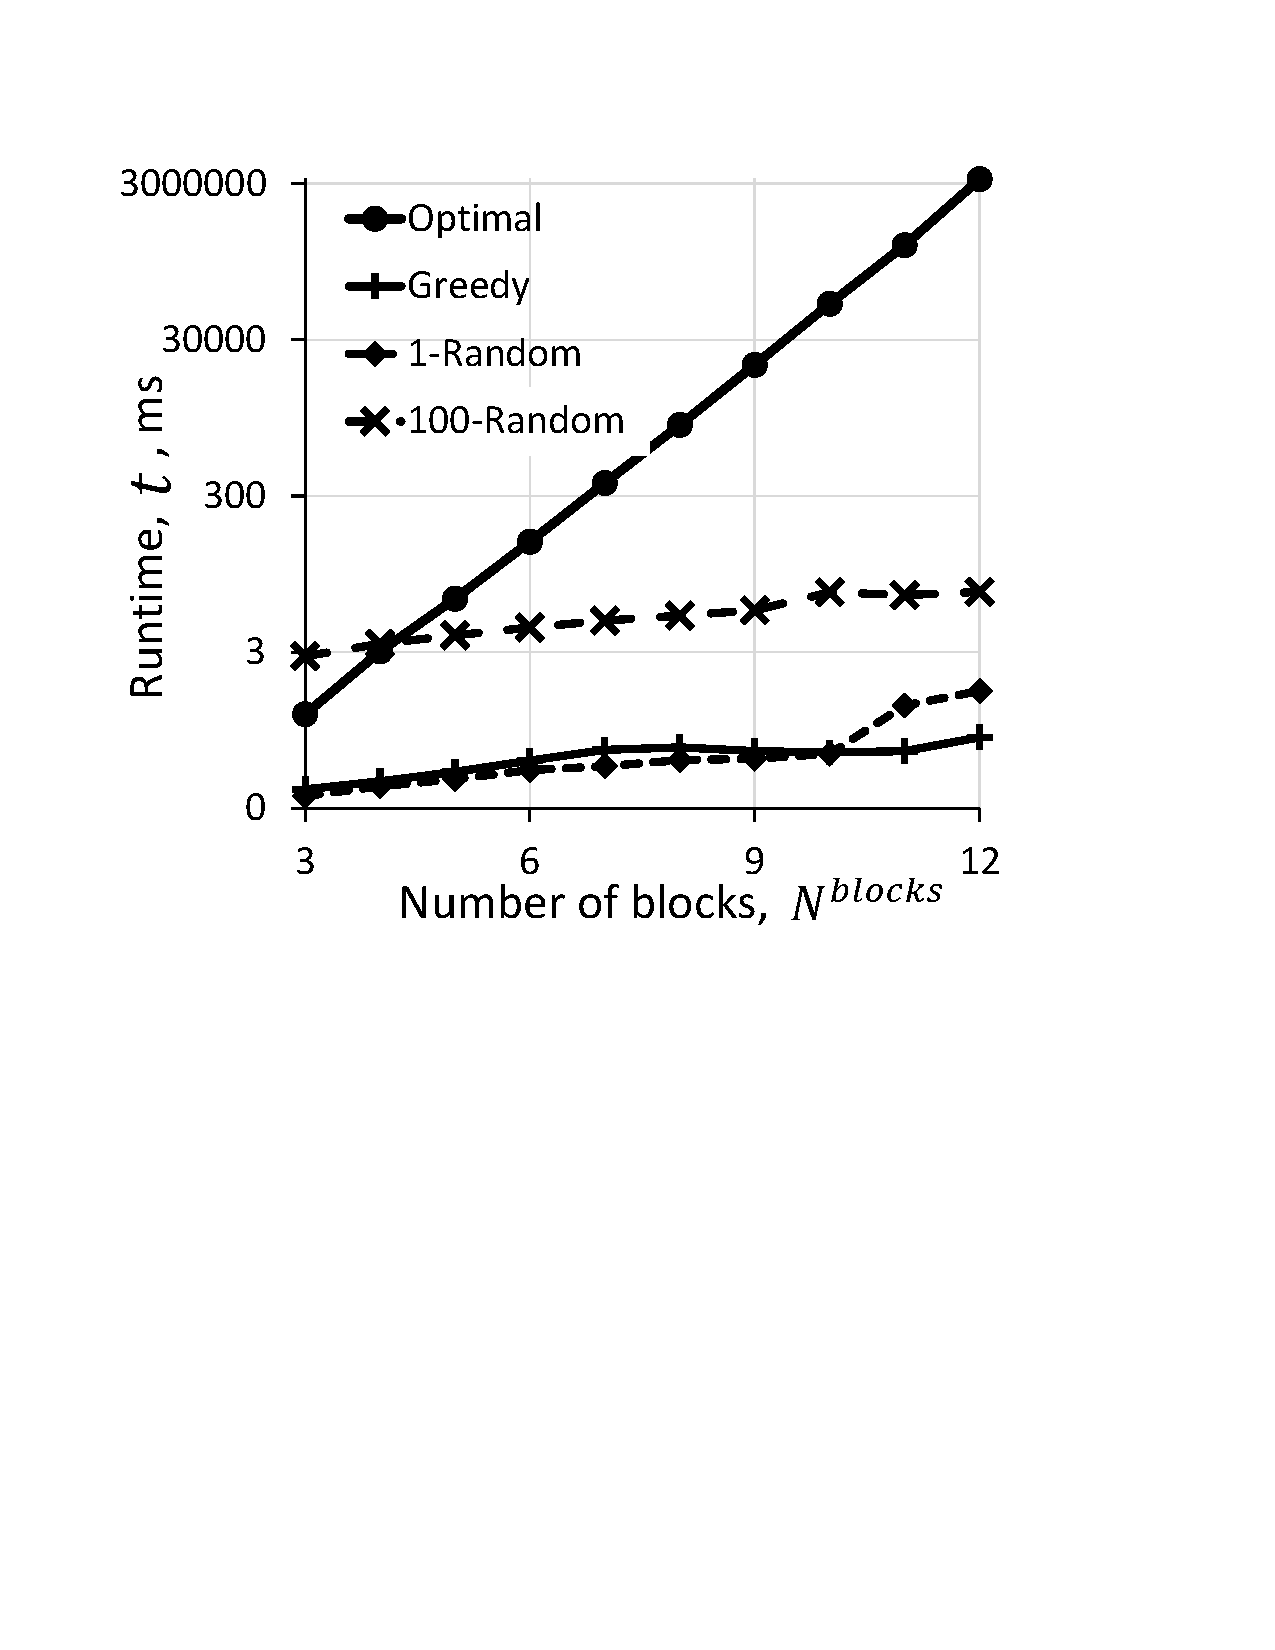
\includegraphics[width=\linewidth]{figs/RuntimeVsBlocks.pdf}
        \caption{Runtime vs. blocks number}
        \label{fig:RuntimeVsBlocks}
    \end{subfigure}
    \hspace{12mm}
    \begin{subfigure}{0.42\textwidth}
        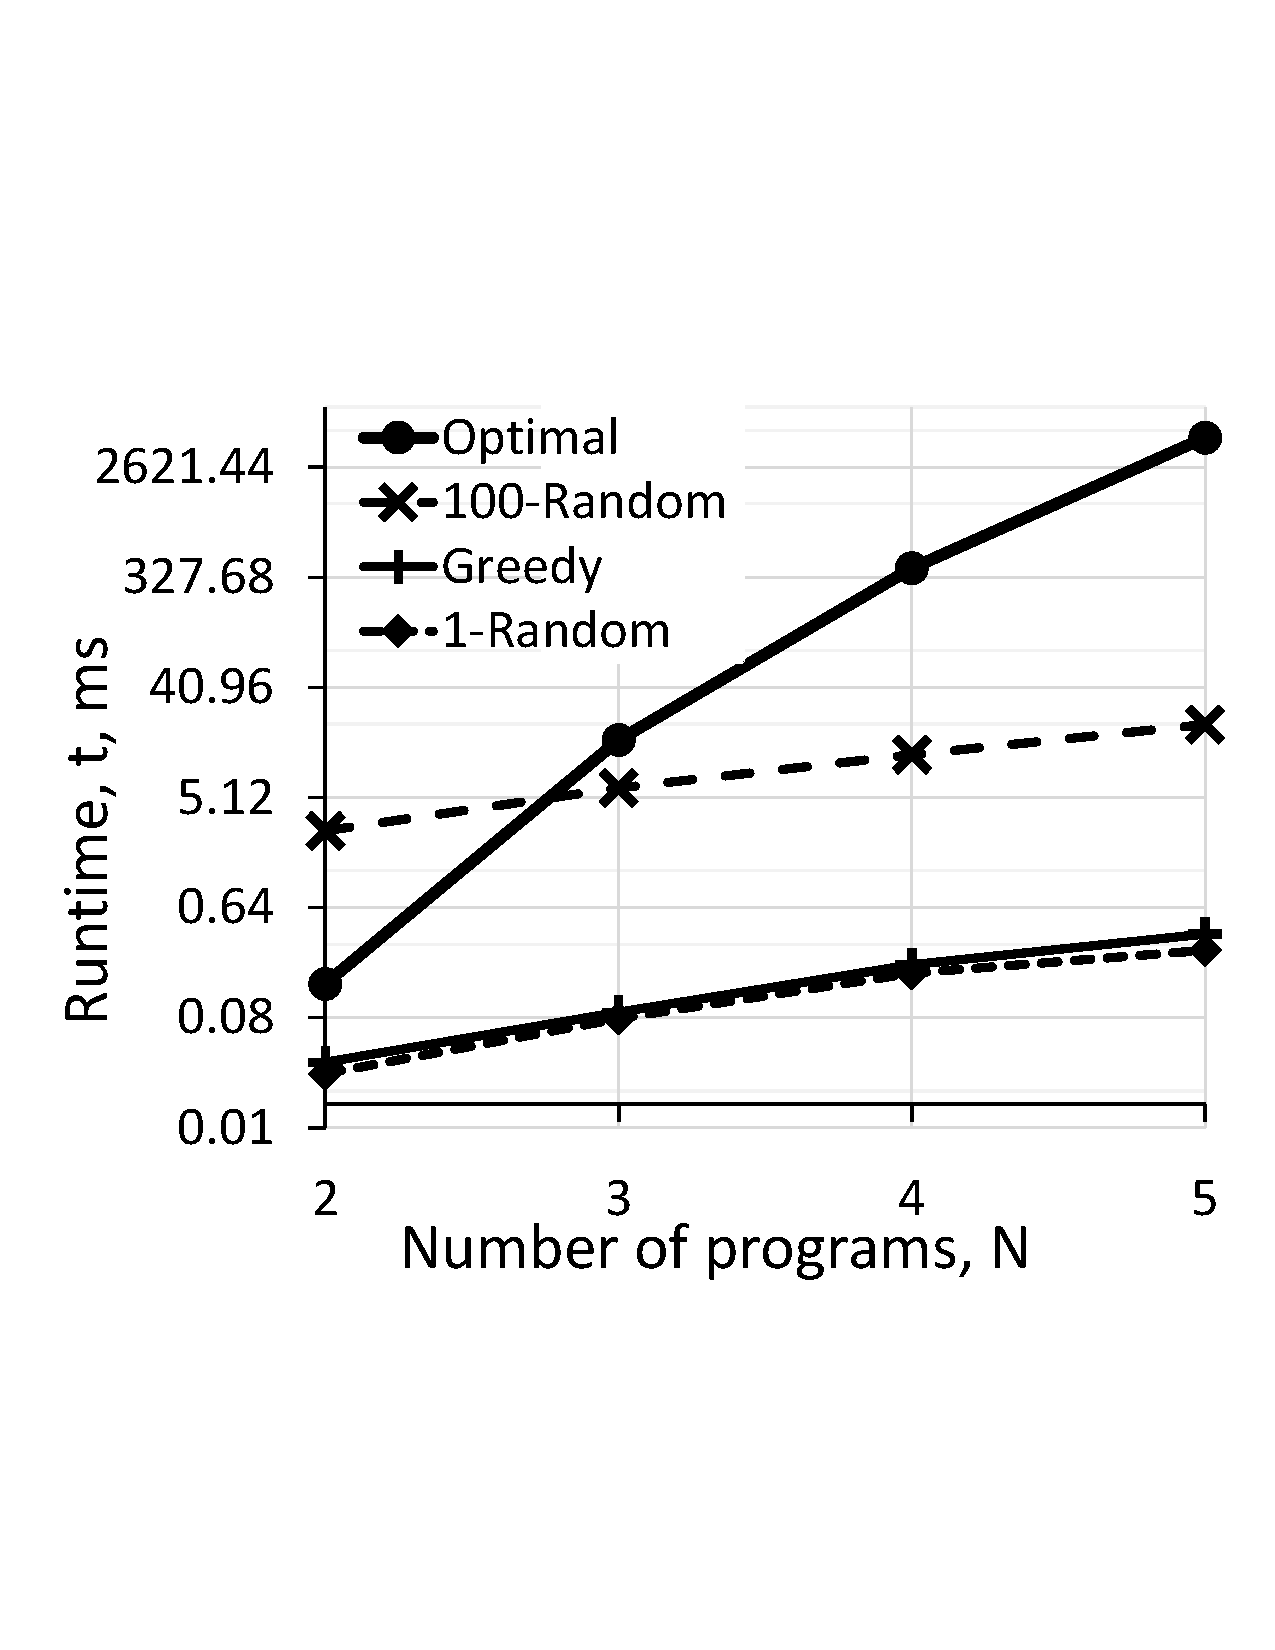
\includegraphics[width=1\linewidth]{figs/RuntimeVsPrograms.pdf}
        \caption{Runtime vs. programs number}
        \label{fig:RuntimeVsPrograms}
    \end{subfigure}
    \caption{Tool runtime dependency of greedy, random walk and optimal schedules}
\end{figure*}




\subsection*{Experiment: Varying program number}
\label{sec:varyingPrograms}

\begin{figure*}
    \centering
    \begin{subfigure}{0.4\textwidth}
        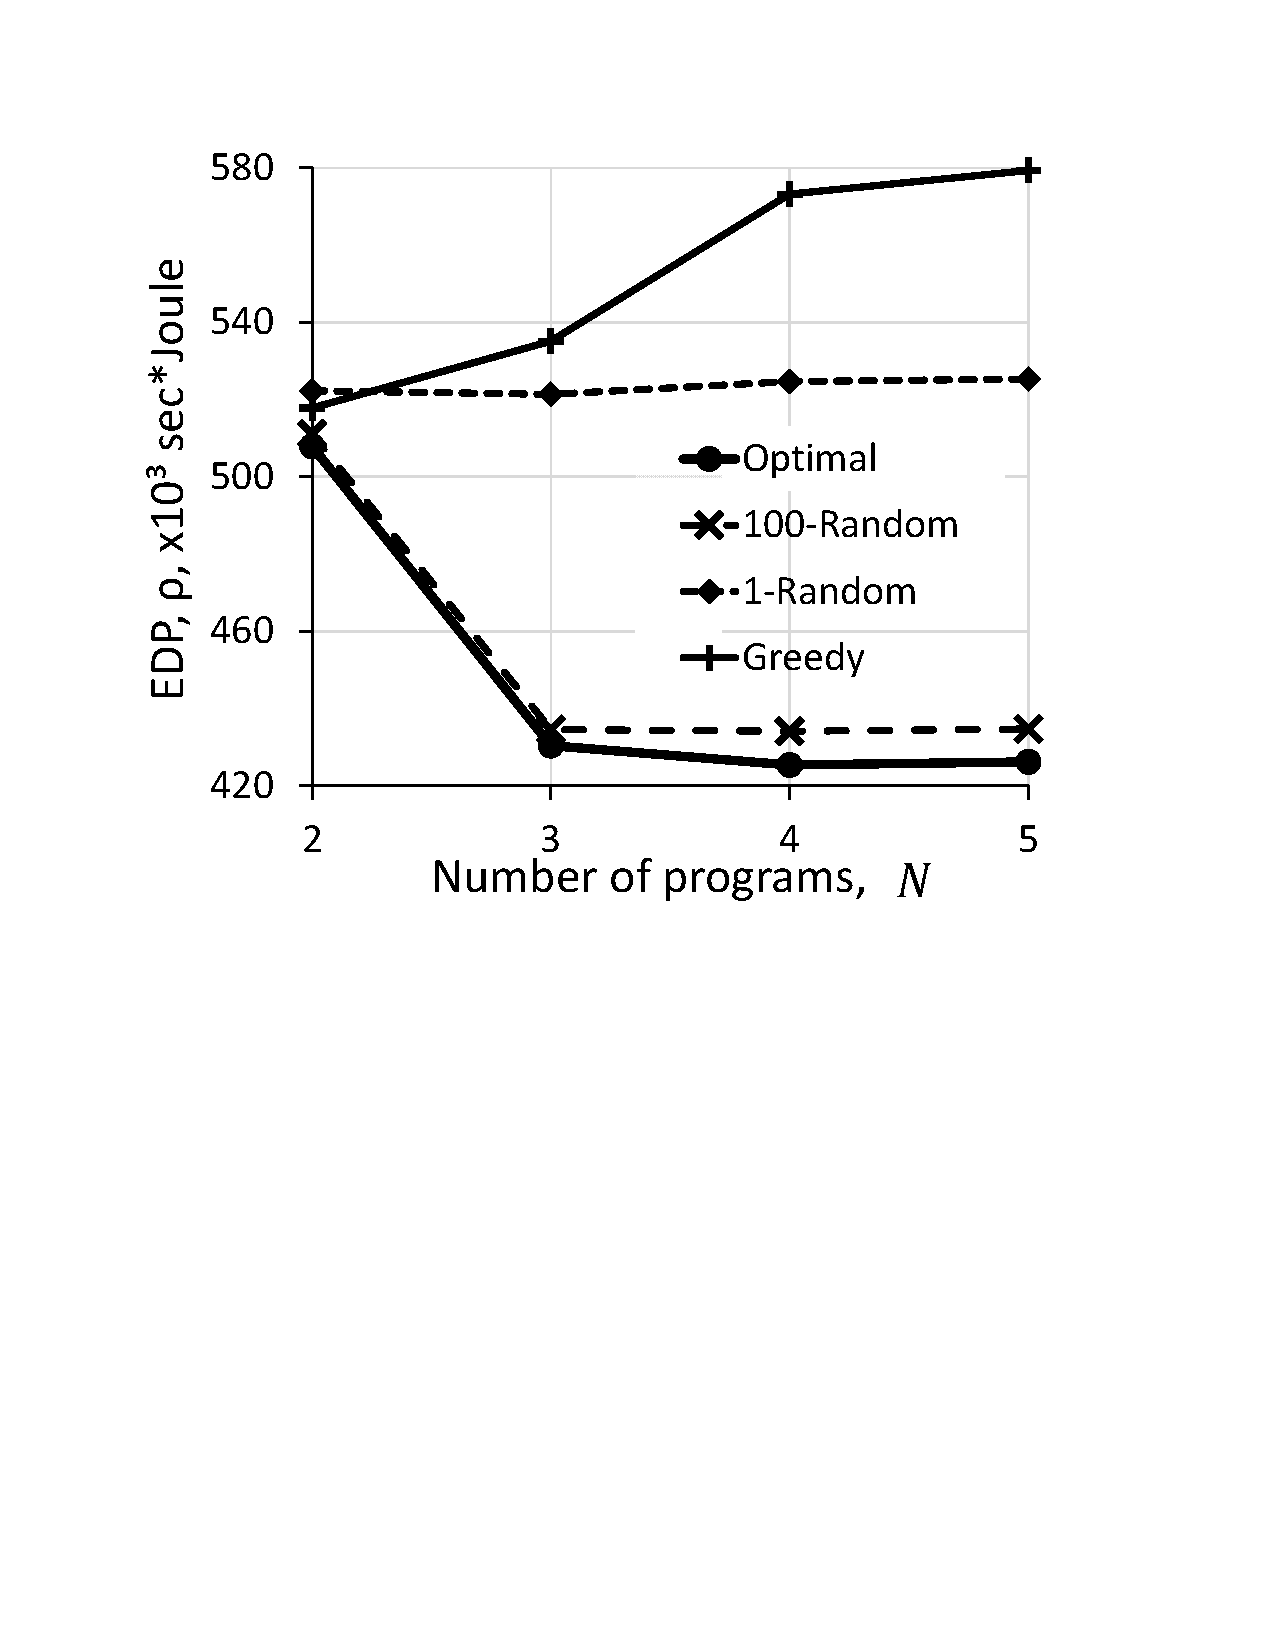
\includegraphics[width=\linewidth]{figs/EDPVsPrograms.pdf}
        \caption{EDP vs. blocks number}
        \label{fig:EDPVsPrograms}
    \end{subfigure}
    \hspace{15mm}
    \begin{subfigure}{0.38\textwidth}
        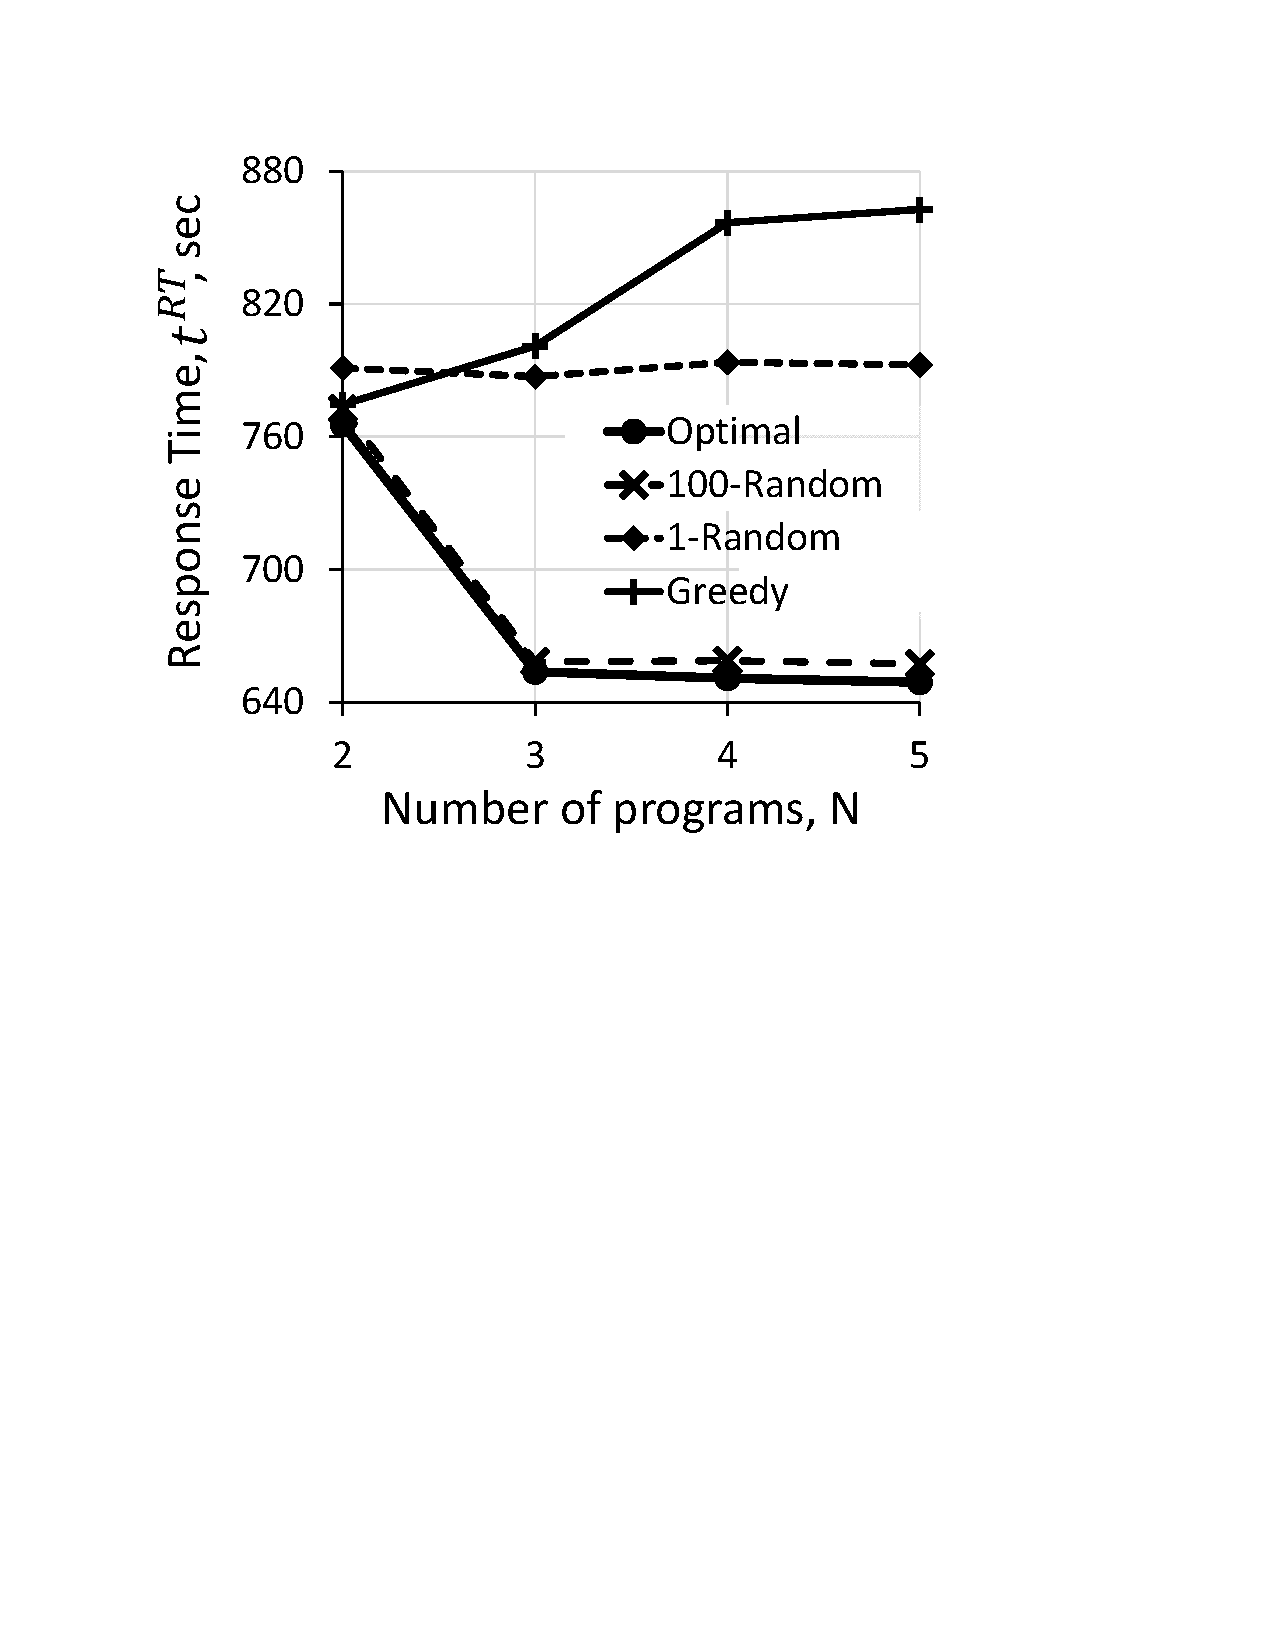
\includegraphics[width=1\linewidth]{figs/RTVsPrograms.pdf}
        \caption{Response time vs. programs number}
        \label{fig:RTVsPrograms}
    \end{subfigure}
    \caption{EDP and programs response time dependencies of greedy, random walk and optimal schedules on number of programs}
\end{figure*}


Fig.~\ref{fig:EDPVsPrograms} illustrates the dependency between EDP $\uprho$ and number of programs $N$. We observe a similar result regarding EDP efficiency: 100-random walk is near-optimal, unlike the single random walk and greedy. The deviation between schedules EDP is again up to 35-40\%. Regarding programs response time in Fig~\ref{fig:RTVsPrograms}, the results are similar to programs EDP.